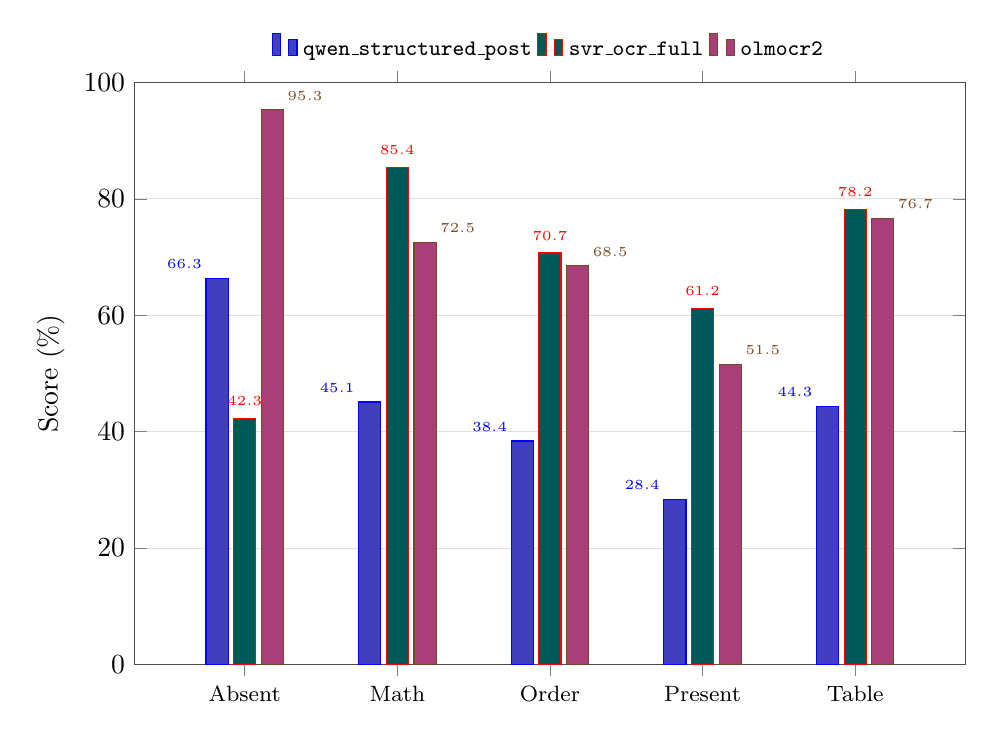
\begin{tikzpicture}
\begin{axis}[
    width=\columnwidth,
    height=0.74\columnwidth,
    ybar,
    bar width=8pt,
    ymin=0,
    ymax=100,
    ylabel={Score (\%)},
    symbolic x coords={Absent,Math,Order,Present,Table},
    xtick=data,
    x tick label style={font=\footnotesize},
    ytick={0,20,40,60,80,100},
    legend style={font=\footnotesize, draw=none, at={(0.5,1.02)}, anchor=south, legend columns=3},
    nodes near coords,
    nodes near coords style={
        font=\tiny,
        /pgf/number format/fixed,
        /pgf/number format/precision=1
    },
    enlarge x limits=0.18,
    axis line style={black!70},
    ymajorgrids=true,
    grid style={draw=black!12}
]
\addplot+[
    fill=blue!50!gray,
    every node near coord/.append style={anchor=south east, xshift=-2pt}
] coordinates {
    (Absent,66.3)
    (Math,45.1)
    (Order,38.4)
    (Present,28.4)
    (Table,44.3)
};
\addplot+[
    fill=teal!70!black,
    every node near coord/.append style={anchor=south, yshift=1pt}
] coordinates {
    (Absent,42.3)
    (Math,85.4)
    (Order,70.7)
    (Present,61.2)
    (Table,78.2)
};
\addplot+[
    fill=magenta!65!black,
    every node near coord/.append style={anchor=south west, xshift=2pt}
] coordinates {
    (Absent,95.3)
    (Math,72.5)
    (Order,68.5)
    (Present,51.5)
    (Table,76.7)
};
\legend{\texttt{qwen\_structured\_post},\texttt{svr\_ocr\_full},\texttt{olmocr2}}
\end{axis}
\end{tikzpicture}
